


\section{Regression}
The basic form of a formula is ``response $\sim$ model".

\section{Analysis of Variance}
Analysis of variance (ANOVA) is a collection of statistical models, and their associated procedures, in which the observed variance in a particular variable is partitioned into components attributable to different sources of variation.



\subsection{Multiple Linear Regression}
The basic model for multiple regression analysis is

\[
y = b_0 + b_1x_1 + \cdots  + b_kx_k + e
\]




\section{Week 6 General Theory Topics}


\subsection{Steps in Building a Predictive Model}
\begin{enumerate}
\item Find the right data
\item Define your error rate
\item Split data into:
\begin{itemize}
\item \textbf{Training Set}
\item \textbf{Testing Set}
\item \textbf{Validation Set} (optional)
\end{itemize}
\item On the training set select predictor variables (features)
\item On the training set generate your predictive model
\item On the training set cross-validate

%\item If no validation - apply 1x to test set
%\item If validation - apply to test set and refine
%\item If validation - apply 1x to validation
\end{enumerate}
%-------------------------------------------------------%
\subsection{Descriptive vs Predictive Models}

\begin{itemize}
	\item A \textbf{descriptive model} is only concerned with modeling the structure in the observed data. It makes sense to train and evaluate it on the same dataset.
	
	\item The \textbf{predictive model} is attempting a much more difficult problem, approximating the true discrimination function from a sample of data. We want to use algorithms that do not pick out and model all of the noise in our sample. We do want to chose algorithms that generalize beyond the observed data. It makes sense that we could only evaluate the ability of the model to generalize from a data sample on data that it had not see before during training.
	
	\item \textbf{IMPORTANT} The best descriptive model is accurate on the observed data. The best predictive model is accurate on unobserved data.
\end{itemize}


\subsection{Overfitting}
\begin{itemize}
	\item The problem with evaluating a predictive model on training data is that it does not inform you on how well the model has generalized to new unseen data.
	
\item 	A model that is selected for its accuracy on the training dataset rather than its accuracy on an unseen test dataset is very likely have lower accuracy on an unseen test dataset. The reason is that the model is not as generalized. It has specalized to the structure in the training dataset. This is called \textbf{overfitting}.
\end{itemize}

\subsection{Cross-Validation and Testing}
%====================================================%
\begin{itemize}
	\item In order to build the best possible mode, we will split our training data into two parts: a training set and a test set. 
	
	\item 	The general idea is as follows. The model parameters (the regression coefficients) are learned using the training set as above. 
	\item The error is evaluated on the test set, and the meta-parameters are adjusted so that this cross-validation error is minimized. 

\end{itemize}	
\subsection{Cross Validation}
%-------------------------------------------------------------------------------------%
\begin{itemize}	
%	\item 	
%	
%	\item	The cross validated set of data is a more honest presentation of the power of the
%	discriminant function than that provided by the original classifications and often produces
%	a poorer outcome. 
	\item The cross validation is often termed a ‘jack-knife’ classification, in that
	it successively classifies \textbf{all cases but one} to develop a predictive model and then
	categorizes the case that was left out. This process is repeated with each case left out in
	turn.This is known as leave-1-out cross validation. 
	
	\item 	This cross validation produces a more reliable function. The argument behind it is that
	one should not use the case you are trying to predict as part of the categorization process.
\end{itemize}



%-----------------------------------------------------------------------------------%
\subsection{Error Rates}

\begin{itemize}
	\item We can evaluate error rates by means of a training sample (to construct build a model) and a test sample.
	
	
	\item 	An optimistic error rate is obtained by reclassifying the training data. (In the \textbf{\textit{training data}} sets, how many cases were misclassified). This is known as the \textbf{apparent error rate}.
	
	
	\item 	The apparent error rate is obtained by using in the training set to estimate
	the error rates. It can be severely optimistically biased, particularly for complex classifiers, and in the presence of over-fitted models.
	
	
	\item	If an independent test sample is used for classifying, we arrive at the  \textbf{true error rate}.The true error rate (or conditional error rate) of a classifier is the expected
	probability of misclassifying a randomly selected pattern.
	It is the error rate of an infinitely large test set drawn from the same distribution as the training data.
\end{itemize}




%---------------------------------------------------------------------------------------%




\subsection{Cross Validation}
\begin{itemize}
\item In a prediction problem, a model is usually given a dataset of known data 
on which training is run (\textit{training dataset}), and a dataset of unknown data (or \textit{first seen data/ testing dataset}) against which testing the model is performed.
\item Cross-validation is mainly used in settings where the goal is prediction, and one wants to estimate how accurately a predictive model will perform in practice, with unseen data.
\item The goal of cross validation is to define a dataset to ``test" the model in the training phase, in order to limit problems like overfitting, give an insight on how the model will generalize to an independent data set (i.e., an unknown dataset, for instance from a real problem), etc.
\item Cross-validation is important in guarding against testing hypotheses suggested by the data (called ``\textbf{\textit{Type III errors}}"), especially where further samples 
are hazardous, costly or impossible to collect 
\end{itemize}
\subsection*{K-fold Cross Validation}
\begin{itemize}
\item In k-fold cross-validation, the original data set is randomly partitioned into $k$ equally sized subsamples (e.g. 10 samples).
 
\item Of the $k$ subsamples, a single subsample is retained as the testing data for testing the model, and the remaining k - 1 subsamples are used as training data. 
\item The cross-validation process is then repeated k times (the folds), with each of the $k$ subsamples used exactly once as the test data. \item The $k$ results from the folds can then be averaged (or otherwise combined) to produce a single estimation.
\item The advantage of this method over repeated random sub-sampling is that all observations are used for both training and testing, and each observation is used for testing exactly once. 
\end{itemize}
%\subsection*{Choosing K - Bias and Variance}
%In general, when using k-fold cross validation, it seems to be the case that:
%\begin{itemize}
%\item A larger k will produce an estimate with smaller bias but potentially higher variance (on top of being computationally expensive)
%\item A smaller k will lead to a smaller variance but may lead to a a biased estimate.
%\end{itemize}
\newpage

\subsection*{Leave-One-Out Cross-Validation}
\begin{itemize}
\item As the name suggests, \textbf{leave-one-out cross-validation}  \textbf{(LOOCV)} involves using a single observation from the original sample as the validation data, and the remaining observations as the training data. 
\item This is repeated such that each observation in the sample is used once as the validation data. 
\item This is the same as a K-fold cross-validation with K being equal to the number of observations in the original sampling, i.e. \textbf{K=n}.
\end{itemize}


\section{Binary Classification}	


\subsection{Category Prediction Table}

\begin{itemize}
	\item It is very common to use binomial logistic regression to predict whether cases can be correctly classified (i.e., predicted) from the independent variables. Therefore, it becomes necessary to have a method to assess the effectiveness of the predicted classification against the actual classification.
	\item  There are many methods to assess this with their usefulness oftening depending on the nature of the study conducted. However, all methods revolve around the observed and predicted classifications, which are presented in the ``\texttt{Classification Table}", as shown below:
	
	
	\begin{figure}
		\centering
		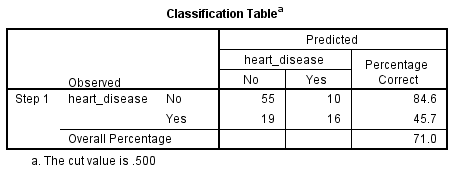
\includegraphics[width=0.8\linewidth]{BLogReg-Table}
	\end{figure}
	
	
	
	\item Firstly, notice that the table has a subscript which states, ``\texttt{The cut value is .500}". This means that if the probability of a case being classified into the ``\textbf{\textit{yes}}" category is greater than .500, then that particular case is classified into the ``\textbf{\textit{yes}}" category. 
	Otherwise, the case is classified as in the ``\textbf{\textit{no}}" category. 
\end{itemize}




\subsection{Classification Table}
Rather than using a goodness-of-fit statistic, we often want to look at the proportion of cases we have managed to classify correctly. For this we need to look at the classification table printed out by SPSS, which tells us how many of the cases where the observed values of the dependent variable were 1 or 0 respectively have
been correctly predicted.

In the Classification table, the columns are the two predicted values of the dependent, while the rows are the two observed (actual) values of the dependent. In a perfect model, all cases will be on the diagonal and the
overall percent correct will be 100\%. In this study, 87.5\% were correctly classified for the take offer group and 92.9\% for the decline offer group. Overall 90\% were correctly classified. This is a considerable improvement on the 53.3\% correct classification with the constant model so we know that the model with predictors is a significantly better mode.
\begin{figure}[h!]
	\begin{center}
		% Requires \usepackage{graphicx}
		\includegraphics[scale=0.6]{Logistic7}\\
		\caption{Classification Table}
	\end{center}
\end{figure}

\subsection{Classification Plot} 
The classification plot or histogram of predicted probabilities
provides a visual demonstration of the correct and incorrect predictions. Also called the `\texttt{classplot}' or the `\texttt{plot of observed groups and predicted probabilities}?,it is another very useful piece of information from the SPSS output when one chooses
\texttt{Classification plots}' under the Options button in the Logistic Regression dialogue box.

\subsection{Interpreting the Classifcation Table}
Whilst the classification table appears to be very simple, it actually provides a lot of important information about your binomial logistic regression result, including:


\begin{itemize}
	\item[A.] The \textbf{percentage accuracy in classification (PAC)}, which reflects the percentage of cases that can be correctly classified as "no" heart disease with the independent variables added (not just the overall model).
	\item[B.] \textbf{Sensitivity}, which is the percentage of cases that had the observed characteristic (e.g., "yes" for heart disease) which were correctly predicted by the model (i.e., true positives).
	\item[C.] \textbf{Specificity}, which is the percentage of cases that did not have the observed characteristic (e.g., "no" for heart disease) and were also correctly predicted as not having the observed characteristic (i.e., true negatives).
	\item[D.] The \textbf{positive predictive value}, which is the percentage of correctly predicted cases "with" the observed characteristic compared to the total number of cases predicted as having the characteristic.
	\item[E.] The \textbf{negative predictive value}, which is the percentage of correctly predicted cases ``without" the observed characteristic compared to the total number of cases predicted as not having the characteristic.
\end{itemize}
%--------------------------------------------------------------------------------------%




%-------------------------------------------------------%

\subsection*{Type III Errors}

\begin{itemize}
\item Type III error is related to hypotheses suggested by the data, if tested using the data set that suggested them, are likely to be accepted even when they are not true. 

\item This is because circular reasoning would be involved: something seems true in the limited data set, therefore we hypothesize that it is true in general, therefore we (wrongly) test it on the same limited data set, which seems to confirm that it is true. 

\item Generating hypotheses based on data already observed, in the absence of testing them on new data, is referred to as \textbf{Post Hoc theorizing}.


\item The correct procedure is to test any hypothesis on a data set that was not used to generate the hypothesis.
\end{itemize}

\end{document}